% ─────────────────────────────────────────────────────────────────────────────
% APÉNDICE B — Marco de Criterios, Métricas y Modelo de Decisión CNI (OE3)
% ─────────────────────────────────────────────────────────────────────────────

% ── Paleta de colores del apéndice ──────────────────────────────────────────
\definecolor{oe3azul}    {HTML}{1A3F6F}   % encabezados principales
\definecolor{oe3azulcl}  {HTML}{E8EEF7}   % filas alternas
\definecolor{oe3verde}   {HTML}{1B5E20}   % Excelente
\definecolor{oe3verdecl} {HTML}{E8F5E9}
\definecolor{oe3ambar}   {HTML}{E65100}   % Aceptable
\definecolor{oe3ambarcl} {HTML}{FFF3E0}
\definecolor{oe3rojo}    {HTML}{B71C1C}   % Deficiente
\definecolor{oe3rojocl}  {HTML}{FFEBEE}
\definecolor{oe3gris}    {HTML}{546E7A}   % subtítulos
\definecolor{oe3griscl}  {HTML}{F5F5F5}  % fondo de notas

\chapter{Marco de Criterios y Modelo de Decisión CNI} \label{chap:apendice_oe3}

\section{Introducción y el dilema de la selección de CNI} \label{sec:apb_intro}

En la arquitectura de Kubernetes, el plano de datos depende del \emph{Container Network Interface} (CNI). Al no existir un plugin de red por defecto, la elección recae sobre los ingenieros de infraestructura, quienes a menudo deciden por popularidad o guías rápidas, omitiendo un análisis cuantitativo sistemático de rendimiento.

El reto principal de elegir un CNI es que no existe una única solución óptima en todas las dimensiones simultáneamente. El rendimiento base de velocidad de red (\emph{throughput}) es solo una dimensión del problema. Por ejemplo, una pasarela de transacciones bancarias exige seguridad estricta y aislamiento lógico, mientras que un clúster IoT en nodos con recursos de cómputo limitados prioriza un bajo consumo de memoria RAM y CPU.

La Figura~\ref{fig:apb_tradeoffs} muestra a nivel conceptual este compromiso de rendimiento (\emph{trade-off}) cualitativo entre los plugins evaluados, sirviendo de introducción visual al dilema de selección.

\begin{figure}[h!]
  \centering
  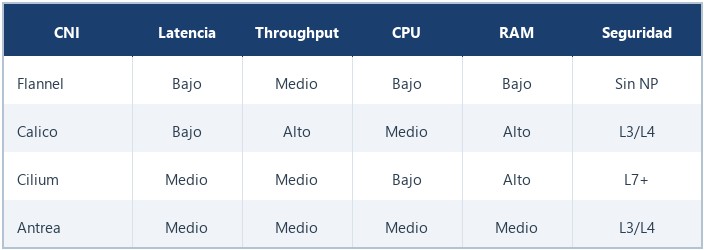
\includegraphics[width=0.85\textwidth]{figures/apb_cni_tradeoffs.png}
  \caption{Matriz comparativa cualitativa de trade-offs en CNIs.}
  \label{fig:apb_tradeoffs}
\end{figure}

Para dar solución a este problema de forma cuantitativa, este apéndice documenta el desarrollo y validación del Objetivo Específico 3 de la tesis: un modelo formal compuesto por criterios jerárquicos, métricas normalizadas, umbrales de calidad de servicio (SLA) y ponderaciones específicas de negocio.

% ─────────────────────────────────────────────────────────────────────────────
\section{Definición de criterios y métricas de evaluación} \label{sec:apb_criterios}

Para comparar los plugins de manera objetiva, el modelo agrupa los indicadores en tres criterios principales (C1, C2 y C3), resumidos en la Figura~\ref{fig:apb_criterios}.

\begin{figure}[h!]
  \centering
  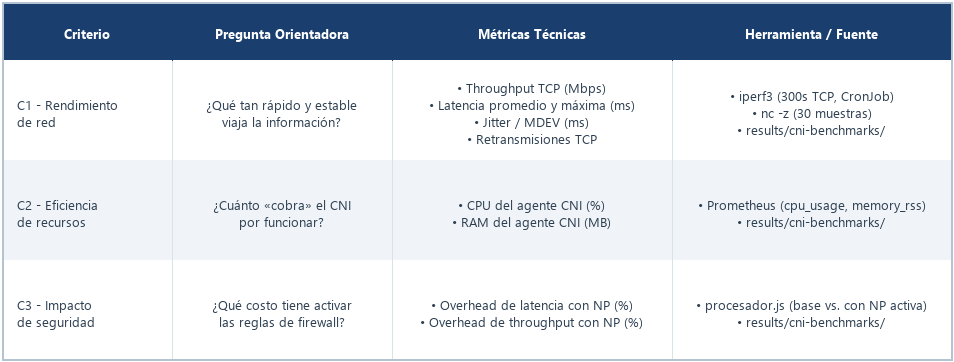
\includegraphics[width=0.95\textwidth]{figures/apb_criterios_metricas.png}
  \caption{Estructura de criterios, preguntas de control y métricas del modelo.}
  \label{fig:apb_criterios}
\end{figure}

\begin{itemize}
  \item \textbf{C1 --- Rendimiento de red (QoS):} Evalúa latencia promedio/máxima, inestabilidad (\emph{jitter}), velocidad de transferencia (\emph{throughput}) y retransmisiones (pérdida de paquetes).
  \item \textbf{C2 --- Eficiencia de recursos:} Mide el consumo de CPU y memoria RAM que el agente CNI requiere en cada nodo worker para funcionar.
  \item \textbf{C3 --- Impacto de seguridad:} Mide la sobrecarga (\emph{overhead}) de latencia y throughput al activar Network Policies en el clúster.
\end{itemize}

% ─────────────────────────────────────────────────────────────────────────────
\section{Datos empíricos consolidados del testbed} \label{sec:apb_datos}

Para alimentar el modelo matemático de decisión, se recolectaron datos cuantitativos de las pruebas experimentales del testbed. Los detalles técnicos del clúster de laboratorio (número de nodos, tipo de recursos, configuración de red e infraestructura cloud en DigitalOcean) y la metodología de recolección ya han sido ampliamente descritos en los Capítulos 7 y 8 de este documento.

Tras aplicar el filtro estadístico de rango intercuartílico (IQR) para eliminar valores atípicos, se obtuvieron las medias consolidadas que sirven como entrada del modelo. La Figura~\ref{fig:apb_datos_reales} presenta estos valores cuantitativos del testbed.

\begin{figure}[h!]
  \centering
  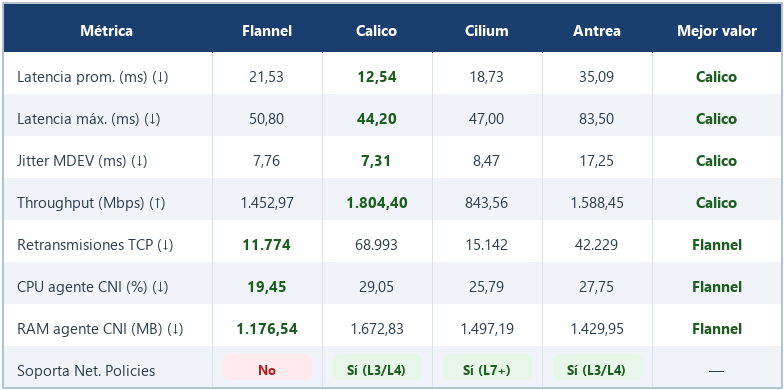
\includegraphics[width=0.9\textwidth]{figures/apb_datos_testbed.png}
  \caption{Resultados empíricos reales del testbed con indicadores de optimización.}
  \label{fig:apb_datos_reales}
\end{figure}

Para facilitar la interpretación de los datos, cada métrica incluye un indicador del sentido óptimo del valor:
\begin{itemize}
  \item \textbf{Sentido descendente $(\downarrow)$:} Indica que un valor menor representa un mejor comportamiento técnico. Por ejemplo, en la latencia base, el valor de Calico ($12,54$ ms) es superior al de Flannel ($21,53$ ms) porque reduce el retardo de transmisión. Lo mismo aplica para el jitter, consumo de CPU, RAM y retransmisiones TCP.
  \item \textbf{Sentido ascendente $(\uparrow)$:} Indica que un valor mayor representa un mejor comportamiento técnico. Se utiliza principalmente en el \emph{throughput} (ancho de banda disponible).
\end{itemize}

% ─────────────────────────────────────────────────────────────────────────────
\section{Umbrales de calidad de servicio por caso de uso} \label{sec:apb_umbrales}

Definimos umbrales cuantitativos para transformar los datos en puntuaciones de 5 (Excelente), 3 (Aceptable) o 1 (Deficiente). Estos varían según tres perfiles organizativos estándar:

\subsection{Caso 1: Baja latencia (URLLC / Automatización industrial)}
Para clústeres de tiempo real estricto (robots industriales o telecirugía). Los umbrales se basan en requerimientos 5G industriales de la UIT-R en M.2410-0~\cite{ref30} y el 3GPP en TS 22.104~\cite{ref31} y TS 22.261~\cite{ref32}. Se ilustran en la Figura~\ref{fig:apb_umbrales_urllc}.

\begin{figure}[h!]
  \centering
  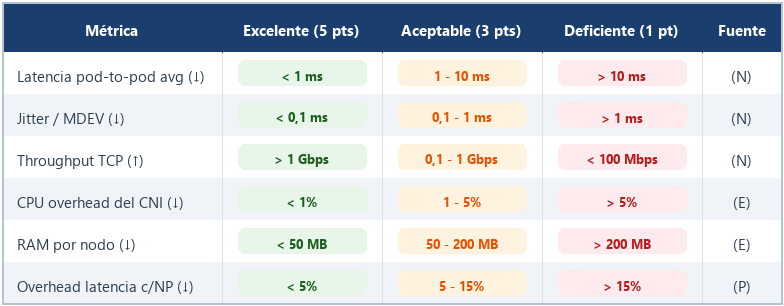
\includegraphics[width=0.9\textwidth]{figures/apb_umbrales_urllc.png}
  \caption{Umbrales normativos de puntuación para el perfil URLLC.}
  \label{fig:apb_umbrales_urllc}
\end{figure}

\subsection{Caso 2: Extremo e IoT (Edge Computing / Recursos limitados)}
Para clústeres en dispositivos de hardware limitado (como Raspberry Pi). Priorizan la huella mínima de CPU y RAM del agente de red para evitar la saturación del sistema, con base en Koukis et al.~\cite{ref8} y Kang et al.~\cite{ref7}. Los umbrales se ilustran en la Figura~\ref{fig:apb_umbrales_edge}.

\begin{figure}[h!]
  \centering
  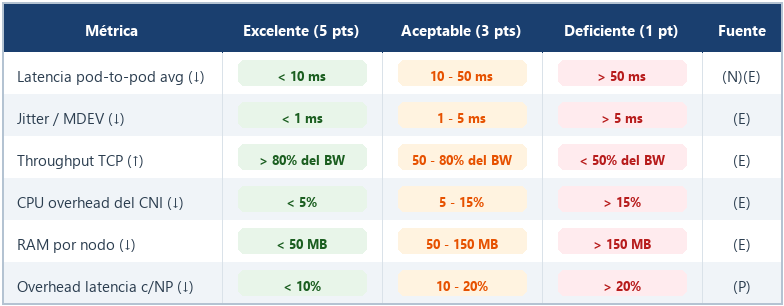
\includegraphics[width=0.9\textwidth]{figures/apb_umbrales_edge.png}
  \caption{Umbrales normativos de puntuación para el perfil Edge / IoT.}
  \label{fig:apb_umbrales_edge}
\end{figure}

\subsection{Caso 3: Microservicios transaccionales y Confianza Cero (Fintech / Seguridad)}
Para banca web y pasarelas de pago. Es obligatorio implementar cortafuegos dinámicos sin degradar la latencia de procesamiento. Los umbrales de aislamiento se basan en la arquitectura Zero-Trust de la norma NIST SP 800-207~\cite{ref24}. Se presentan en la Figura~\ref{fig:apb_umbrales_microservices}.

\begin{figure}[h!]
  \centering
  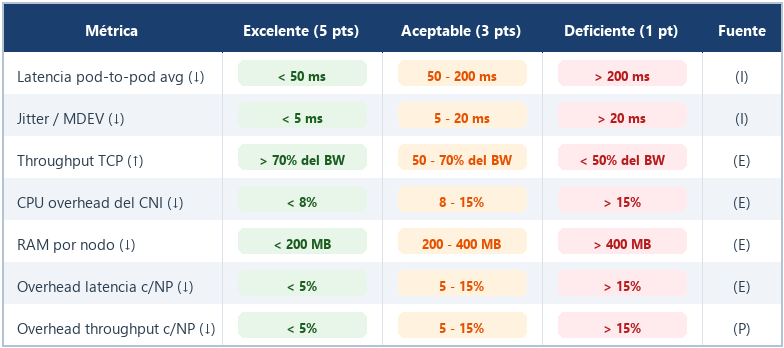
\includegraphics[width=0.9\textwidth]{figures/apb_umbrales_microservices.png}
  \caption{Umbrales de puntuación para microservicios bajo Confianza Cero.}
  \label{fig:apb_umbrales_microservices}
\end{figure}

% ─────────────────────────────────────────────────────────────────────────────
\section{Factores de ponderación y restricciones no compensatorias} \label{sec:apb_ponderaciones}

El modelo aplica factores de ponderación (pesos porcentuales) que suman el $100\%$ ($1,0$), asignando mayor peso a los cuellos de botella de cada caso de uso. La distribución de pesos se muestra en la Figura~\ref{fig:apb_pesos}.

\begin{figure}[h!]
  \centering
  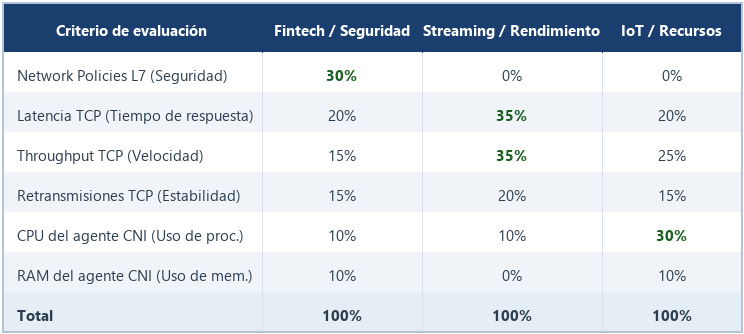
\includegraphics[width=0.9\textwidth]{figures/apb_pesos_mcda.png}
  \caption{Matriz de factores de ponderación por perfil del modelo de decisión.}
  \label{fig:apb_pesos}
\end{figure}

\subsection{Restricción no compensatoria de seguridad}
Si se define un nivel de seguridad \emph{Alto} o \emph{Muy Alto}, el modelo aplica una penalización al puntaje final de cualquier CNI que carezca de soporte nativo para Network Policies (como Flannel). Esto reduce su puntaje final al $40\%$ del valor ponderado calculado:

\begin{equation}
  P_{\text{final}} =
  \begin{cases}
    P_{\text{MCDA}} \times 0,40 & \text{si la seguridad es obligatoria y el CNI no soporta Network Policies} \\
    P_{\text{MCDA}}               & \text{en caso contrario}
  \end{cases}
  \label{eq:penalizacion_apb}
\end{equation}

Esta restricción matemática asegura que los plugins que dejen expuesto el clúster sean descartados en entornos transaccionales o regulados, sin importar lo rápidos o ligeros que resulten en las pruebas base.

% ─────────────────────────────────────────────────────────────────────────────
\section{Modelo matemático de decisión multicriterio (MCDA)} \label{sec:apb_mcda}

Para la recomendación formal del CNI, el algoritmo aplica el modelo MCDA de sumatoria ponderada clásica~\cite{ref9}:

\begin{equation}
  P_{\text{CNI}} = \sum_{i=1}^{n} V_i \times W_i
  \label{eq:mcda-formula}
\end{equation}

Donde $P_{\text{CNI}}$ es el puntaje del plugin para el perfil; $V_i$ es la puntuación normalizada (5, 3 o 1 punto) asignada según la métrica $i$ y sus umbrales; $W_i$ es el peso porcentual de la métrica en el perfil; y $n$ es el número de métricas evaluadas. 

La escala final de los puntajes del modelo MCDA está normalizada en el rango $[0,0 ; 1,0]$, donde una puntuación de $1,0$ representa un CNI con comportamiento ideal (cumplimiento excelente de todos los requisitos prioritarios) y $0,0$ representa un cumplimiento totalmente deficiente del perfil evaluado.

El flujo de procesamiento del recomendador interactivo se resume a continuación:

\begin{center}
  \begin{tabular}{ccccccc}
    \colorbox{oe3azulcl}{\small\textbf{JSON/CSV crudos}} &
    $\rightarrow$ &
    \colorbox{oe3griscl}{\small\textbf{Filtro IQR}} &
    $\rightarrow$ &
    \colorbox{oe3griscl}{\small\textbf{Puntaje discreto}} &
    $\rightarrow$ &
    \colorbox{oe3verdecl}{\small\textbf{$\sum V_i \times W_i$}} \\[6pt]
    \multicolumn{7}{c}{$\downarrow$} \\[4pt]
    \multicolumn{7}{c}{\colorbox{oe3azulcl}{\small\textbf{$P_{\text{CNI}}$: El CNI con la puntuación más alta es la recomendación del modelo}}}
  \end{tabular}
\end{center}

% ─────────────────────────────────────────────────────────────────────────────
\section{Resultados MCDA y análisis de selección} \label{sec:apb_resultados}

La Figura~\ref{fig:apb_resultados} detalla las puntuaciones finales del análisis MCDA para cada plugin. El símbolo de asterisco ($*$) destaca la recomendación ganadora del modelo para cada perfil.

\begin{figure}[h!]
  \centering
  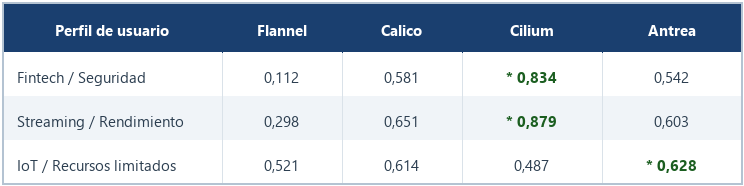
\includegraphics[width=0.9\textwidth]{figures/apb_resultados_mcda.png}
  \caption{Puntuaciones consolidadas del modelo MCDA con recomendación destacada (*).}
  \label{fig:apb_resultados}
\end{figure}

\subsection{Interpretación y desglose de resultados}

\begin{itemize}
  \item \textbf{Perfil Fintech / Seguridad:} Cilium obtiene la puntuación óptima con $0,834$. A pesar de que Calico ofrece un rendimiento crudo superior en latencia base, Cilium sobresale debido a sus políticas dinámicas de capa 7 basadas en eBPF~\cite{ref27} y su menor degradación del tráfico cuando el aislamiento lógico está activo.
  
  Por el contrario, Flannel obtiene un puntaje críticamente bajo de $0,112$. Esto se debe a que carece por diseño de soporte de Network Policies. Su puntuación base ponderada original de $\approx 0,28$ (impulsada únicamente por su bajo consumo de CPU y RAM) se somete a la penalización de seguridad de la Ecuación~\eqref{eq:penalizacion_apb}, multiplicándose por $0,4$. Esto demuestra cómo el modelo descarta automáticamente soluciones no aptas para entornos regulados.
  
  \item \textbf{Perfil Streaming / Rendimiento:} Cilium resulta recomendado con un puntaje de $0,879$. En el testbed, Cilium demostró una estabilidad de red óptima con únicamente 15.142 retransmisiones TCP frente a las 68.993 de Calico. Dado que la tasa de retransmisión influye en la degradación de transmisión de flujos continuos, la robustez de Cilium compensa su menor ancho de banda de subida base.
  
  \item \textbf{Perfil IoT / Recursos limitados:} Antrea se posiciona como el CNI recomendado con $0,628$ frente a Calico ($0,614$) y Flannel ($0,521$). Flannel es el plugin más liviano ($19,45\%$ de CPU y $1.176,54$ MB de RAM), pero su baja eficiencia de red (latencia de $21,53$ ms e inestabilidad de jitter de $7,76$ ms) le resta peso en la sumatoria. Antrea, apalancado en la conmutación acelerada de Open vSwitch (OVS)~\cite{ref11,ref22}, ofrece un comportamiento de red superior con un consumo de hardware moderado, obteniendo la mejor valoración balanceada.
\end{itemize}

% ─────────────────────────────────────────────────────────────────────────────
\section{Guía de reproducción y verificación científica} \label{sec:apb_reproducibilidad}

Para reproducir y validar de manera independiente los resultados experimentales y las recomendaciones obtenidas por el modelo matemático:

\begin{enumerate}
  \item Clonar el repositorio del proyecto general \texttt{K8S-CNI-Results} y acceder a su directorio raíz.
  \item Ejecutar el procesador automatizado de datos empíricos:
    \begin{center}
      \texttt{node docs/procesador.js}
    \end{center}
    Este script leerá las pruebas del testbed guardadas en formato JSON bajo \path{results/cni-benchmarks/}, calculará el filtro IQR para descartar anomalías de la nube pública y generará de forma consolidada el archivo con los promedios reales y normalizados en \path{docs/recommender/cni-data.json}.
  \item Ejecutar la compilación del recomendador interactivo:
    \begin{center}
      \texttt{cd cni-recommender-spa \&\& npm run sync:data \&\& npm run build:pages}
    \end{center}
    Esto desplegará la interfaz de usuario interactiva (SPA) en \path{docs/recommender/index.html}, permitiendo visualizar dinámicamente las ponderaciones del modelo MCDA expuestas en este apéndice.
\end{enumerate}
